\documentclass{aruno-gist}

\usepackage{mylayout}

\webversionfalse

%% Details of the book
%% ===================

\title{Dhammapada-Reflexionen}
\subtitle{52 Verse aus dem Dhammapada mit Kommentaren von Ajahn Munindo}
\author{Ajahn Munindo}
\date{}
% TODO confirm number of copies
\editionInfo{\textit{Zweite Auflage}, X,XXX Kopien, gedruckt in Malaysia, 2018}
% TODO isbn
\ISBN{000-0-000000-00-0}

% \hyphenation{prep-a-ra-tion belief attrac-tive under-stand-ing moment}

\begin{document}

\ifwebversion
\webcover{%
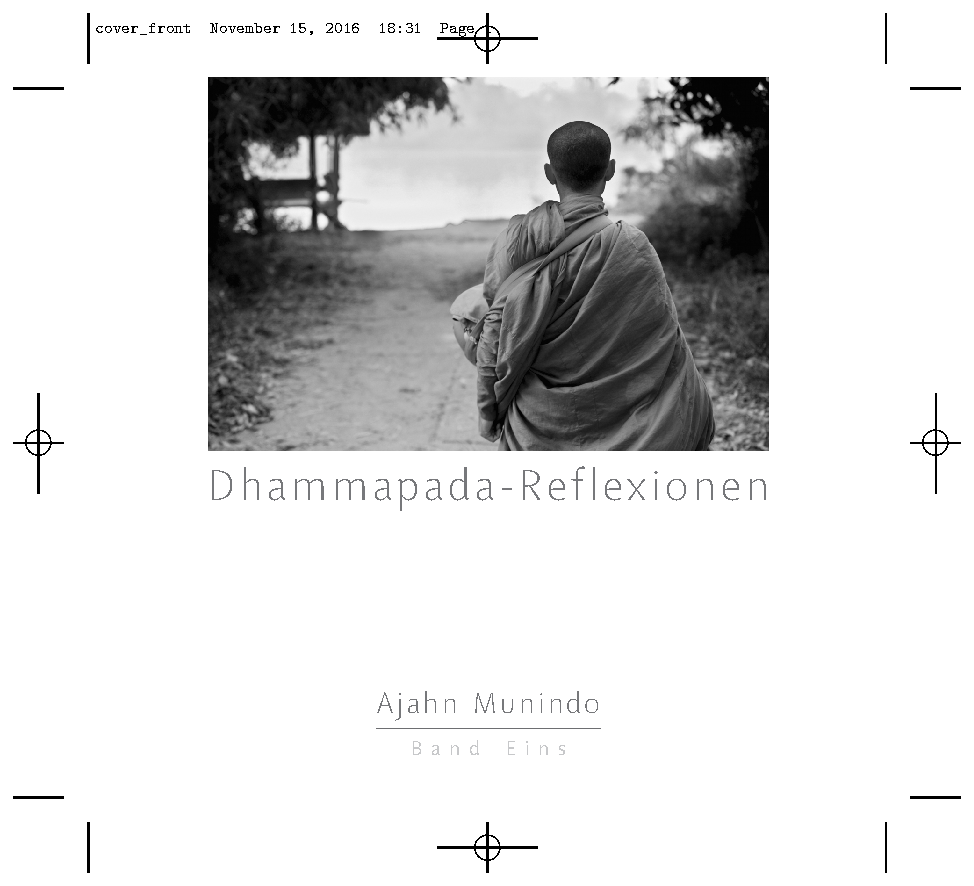
\includegraphics[width=\paperwidth]{./cover_front.pdf}
}
\else

% Gray color page
% Pantone 423M
% CMYK 22, 14, 18, 45

\thispagestyle{empty}
\mbox{}
\pagecolor{frontgray}
\newpage
\thispagestyle{empty}
\pagecolor{white}
\mbox{}
\newpage

\fi

%% Frontmatter
%% ===========

\frontmatter*
\pagestyle{empty}

\midsloppy

\cleartorecto
\begin{quotepage}{60mm}
\centering
\itshape
Beim Hören wahrer Lehren werden\\
die Herzen jener, die empfänglich sind,\\
ruhig wie ein See, tief, klar und still.

{\smaller Dhammapada Vers 82}
\end{quotepage}



\cleartoverso
\begin{quotepage}{80mm}
\centering
\emph{Widmungen}

Wir möchten uns für die Unterstützung bei all denjenigen bedanken, die bei der
Zusammenstellung dieses Buches geholfen haben, vor allem bei der Gruppe
Kataññutā aus Malaysia, Singapur und Australien dafür, dass sie den Druck des
Buches ermöglicht hat.

Besonderer Dank gilt auch Dr Ute Weber und Adelbert Buffy für ihre Hilfe bei den
Korrekturen und Verbesserungen der Übersetzung für diese zweite, überarbeitete
Auflage.

\end{quotepage}



\cleartorecto
\thispagestyle{empty}
\vspace*{5em}
\newlength\titleLength
\newlength\xheight

{\centering

\settowidth{\titleLength}{%
  {\Large\chapterTitleFont\scshape\MakeLowercase{\thetitle}}%
}

{\Large\chapterTitleFont\scshape\MakeLowercase{\thetitle}}\\[0.3\baselineskip]
\setlength{\xheight}{\heightof{X}}
\raisebox{0.5\xheight}{\color[gray]{0.4}\rule{\titleLength}{0.1pt}}\\[0.3\baselineskip]
{\itshape
\thesubtitle}

\vfill

\theauthor

\vspace*{5em}

}




\cleartoverso
\thispagestyle{empty}
{\copyrightsize\setlength{\parskip}{0.5\baselineskip}\setlength{\parindent}{0em}%
\raggedright%
\shaker\color[gray]{0.3}

\thetitle\\
von \theauthor

Zweite, überarbeitete Auflage der Übersetzung.

Veröffentlicht bei Aruno Publications,\\
Northumberland, Vereinigtes Königreich

Kontakt Aruno Publications at \href{http://ratanagiri.org.uk/}{www.ratanagiri.org.uk}\\
Dieses Buch ist zum freien Herunterladen verfügbar\\
\href{http://fsbooks.org/}{www.fsbooks.org}

Originaltitel: Dhammapada Reflections

ISBN \theISBN

Copyright \copyright\ 2009 HARNHAM BUDDHIST MONASTERY TRUST

\pali{Sabbadānaṃ dhammadānaṃ jinati}\\
`Das Geschenk des Dhammas übertrifft alle Gaben'

Foto von Andrew Binkley\\
\href{http://andrewbinkley.com}{www.andrewbinkley.com}

{\tiny
Dieses Werk bzw. Inhalt steht unter einer Creative Commons\\
Namensnennung-NichtKommerziell-KeineBearbeitung 3.0 Unported Lizenz.\\
\href{http://creativecommons.org/licenses/by-nc-nd/3.0/deed.de}{http://creativecommons.org/licenses/by-nc-nd/3.0/deed.de}

Siehe Seite \pageref{copyright-details} für mehr Details über Ihre Rechte und Restriktionen unter dieser Lizenz.

Produziert mit dem \LaTeX\ Satzsystem. Der Haupttext ist in Shaker Pali gesetzt, von Jeremy Tankard erstellt.

\theEditionInfo

}}



\chapterstyle{frontmatter}

\chapter{Vorwort}

Für Laien in buddhistischen Ländern ist es seit langem Tradition an
jedem Neu- und Vollmond ein Kloster am Ort zu besuchen, um sich einen
Dhamma-Vortrag anzuhören. Sogar der Buddha selbst ermutigte seine Sangha
diese vierzehntägige Praxis zu pflegen. Als mir vorgeschlagen wurde, das
Internet zu nutzen, um zu jedem Neu- und Vollmond kurze
Dhamma-Reflexionen zu verschicken, war ich von dieser Idee zunächst
nicht überzeugt, beschloss dann aber doch es auszuprobieren. Obwohl wir
in einer Welt leben, in der die Mondphasen keine große Bedeutung mehr
haben, helfen solche Reflexionen auch heute noch vielen Menschen, an die
alte Tradition, der wir angehören, erinnert zu werden.

Im September 2007 begannen wir Verse aus dem Dhammapada zu verschicken,
die wir aus \emph{A Dhammapada for Contemplation} (2006) ausgewählt hatten. An
jedem `Mond-Tag' wurde ein Vers angeboten, der durch einen kurzen
Kommentar erläutert wurde. Dieses Programm ist mittlerweile durch
Mundpropaganda und weitergeleitete E-Mails recht bekannt geworden. Ich
höre von Menschen aus verschiedenen Teilen der Welt, dass sie es
schätzen, von Zeit zu Zeit eine Erinnerung an eine alte Lebensweise zu
erhalten, während sie ihrem geschäftigen Leben nachgehen. Andere freuen
sich an jedem Neu- und Vollmond darauf, ihre E-Mails zu öffnen, wenn sie
abends von der Arbeit heimkommen. Diese Dhamma-Reflexionen werden privat
genutzt und vielfach kopiert, übersetzt und herumgereicht. Ich habe auch
gehört, dass sie des Öfteren als Diskussionsgrundlage für
Meditationsgruppen dienen. Indem ich meine persönlichen Reflexionen auf
diesem Wege mit Anderen teile, möchte ich sie ermutigen, ihre eigenen
kontemplativen Fähigkeiten zu nutzen. Es scheint unter praktizierenden
Buddhisten im Westen die Tendenz zu geben, Frieden und Verständnis
finden zu wollen, indem sie versuchen ihre Gedanken anzuhalten. Doch der
Buddha spricht davon, dass wir die wahre Natur unseres Geistes durch
`yoniso manasikara' oder weises Betrachten erkennen werden, nicht allein
dadurch, dass wir aufhören zu denken.

Ich möchte mich bei allen bedanken, die bei der Vorbereitung dieses
Materials geholfen haben. Für die Dhammapada-Verse habe ich verschiedene
verlässliche Übersetzungen herangezogen. Insbesondere habe ich die
Arbeit von Ven. Narada Thera (BMS 1978), Ven. Ananda Maitreya Thera
(Lotsawa 1988), Daw Tin Mya und den Herausgebern der burmesischen
Pitaka-Vereinigung (1987) und von Ajahn Thanissaro verwendet. Für die
(kommentariell) überlieferten Geschichten zu den Versen habe ich auch
die Internet-Seite www.tipitaka.net als Quelle genutzt.

Als ich von zahlreichen Lesern gehört hatte, dass eine Buch-Version
dieser Reflexionen nützlich wäre, habe ich mich an meinen guten Freund
Ron Lumsden gewandt. Sein beachtliches Geschick für redaktionelle
Bearbeitung hat dazu beigetragen, meine Arbeit einem größeren Publikum
zugänglich zu machen.

Möge das Gute, das aus der Zusammenstellung dieses kleinen Büchleins
entsteht, mit allen, die an der Produktion und dem Sponsoring beteiligt
waren, geteilt werden. Mögen alle, die den Weg suchen, ihn finden und
die Freiheit am Ende des Weges erleben. Mögen alle Wesen den Weg suchen.

\bigskip

{\par\raggedleft
Bhikkhu Munindo\\
Aruna Ratanagiri, Regenzeitretreat 2009
\par}



%% Main matter
%% ===========

\mainmatter*

\cleartorecto
\thispagestyle{empty}
{\centering

\vspace*{0.6\textheight}
{\chapNameFont\LARGE\color{chaptitle}\soChapter{Dhammapada-Reflexionen}}

}



\setcounter{chapter}{0}
\setcounter{page}{1}
\pagestyle{normalpage}
\chapterstyle{mainmatter}

\setlength{\parskip}{0.6\baselineskip}
\setlength{\parindent}{0pt}

%% == 1 ==

\begin{dhpVerse}{87-88}
\label{dhp-87}\label{dhp-88}
Mit einem Bild der Freiheit als Ziel vor Augen\\ 
wendet sich der Weise von der Dunkelheit ab, \\ 
strebt dem Licht zu, lässt belanglose Sicherheit\\ 
zurück und sucht Freiheit von Anhaftung.\\ 
Eine solche Befreiung anzustreben\\ 
ist schwierig und selten,\\ 
dennoch wird der Weise sie suchen,\\ 
die Hindernisse überwinden,\\ 
Herz und Geist veredelnd. 
\end{dhpVerse}

\begin{dhpRefl}

Der Buddha führt uns mit Bildern das Ziel vor Augen, um uns zu ermutigen und
unsere Bemühungen zu unterstützen, das loszulassen, was uns hindert und
begrenzt. Wenn wir zu stark an solchen Bildern festhalten, können wir das Hier
und Jetzt aus den Augen verlieren – anstatt wirklich in die Praxis
einzutauchen, stellen wir sie uns nur vor. Wenn wir es nicht schaffen, das
Ziel mit Nachdruck zu verfolgen, können wir uns in der Zerstreuung von
Sinnesobjekten – angenehmen wie unangenehmen – verlieren. Wahre Freiheit zu
erlangen ist schwierig, aber bedenke, wie viel Leid uns bevorsteht, wenn wir
nicht praktizieren. Durch weise Reflexion gelingt es uns, die dunklen und
schwierigen Zeiten zu ertragen. Wenn das Licht dann zurückkehrt, schätzen wir
es und werden uns gewahr, wie wir die Wahrheit noch vollkommener lieben
können.

\end{dhpRefl}


\backmatter

\bookmarksetup{startatroot}

\chapterstyle{backmatter}
\newgeometry{vmargin=15mm, hmargin=10mm}

% FIXME: remove page number before index page

\chapter{Inhaltsverzeichnis}

{\smaller
\setlength{\parskip}{0pt}
\setlength{\parindent}{0pt}

\begin{longtable}[c]{llr}
v. 1 & Alle Gemütszustände werden durch den Geist bestimmt. & \pageref{dhp-1}\\
v. 2 & Alle Gemütszustände werden durch den Geist bestimmt. & \pageref{dhp-2}\\
v. 3-4 & Wenn wir an Gedanken festhalten wie: & \pageref{dhp-3}\\
v. 5 & Niemals wird Hass durch Hass besiegt, & \pageref{dhp-5}\\
v. 6 & Jene, die streitsüchtig sind, & \pageref{dhp-6}\\
v. 8 & So wie ein stürmischer Wind & \pageref{dhp-8}\\
v. 14 & So wie Regen ein gut gedecktes Strohdach & \pageref{dhp-14}\\
v. 20 & Nur ein wenig über den Dhamma wissend, & \pageref{dhp-20}\\
v. 49 & Wie eine Biene Nektar sammelt & \pageref{dhp-49}\\
v. 58-9 & Wie eine wohlriechende und prachtvolle Lotosblume & \pageref{dhp-58}\\
v. 76 & Segen kann nur von der Gemeinschaft & \pageref{dhp-76}\\
v. 78 & Suche nicht die Gemeinschaft & \pageref{dhp-78}\\
v. 82 & Beim Hören wahrer Lehren werden & \pageref{dhp-82}\\
v. 87-8 & Mit einem Bild der Freiheit als Ziel vor Augen & \pageref{dhp-87}\\
v. 91 & Wachsam gegenüber den Bedürfnissen der Reise, & \pageref{dhp-91}\\
v. 95 & Da sind jene, die entdecken, & \pageref{dhp-95}\\
v. 104-5 & Seiner selbst Herr zu sein, & \pageref{dhp-104}\\
v. 118 & Hat man eine gute Tat vollbracht, & \pageref{dhp-118}\\
v. 120 & Sogar jene, die ein tugendhaftes Leben führen, & \pageref{dhp-120}\\
v. 122 & Ignoriere nicht den Effekt Rechter Handlung, & \pageref{dhp-122}\\
v. 130 & Hat man Einfühlungsvermögen für andere, & \pageref{dhp-130}\\
v. 134 & Spricht man derb zu dir, & \pageref{dhp-134}\\
v. 142 & Eine extravagante äußere Erscheinung & \pageref{dhp-142}\\
v. 143 & Ein gut trainiertes Pferd gibt keinen Anlass & \pageref{dhp-143}\\
v. 145 & Jene, die Kanäle bauen, & \pageref{dhp-145}\\
v. 146 & Was soll das Gelächter? & \pageref{dhp-146}\\
v. 153-4 & Für viele Leben bin ich, suchend nach dem Hausbauer, & \pageref{dhp-153}\\
v. 162 & Übelgesinnte handeln sich selbst gegenüber & \pageref{dhp-162}\\
v. 169 & Lebe dein Leben im Einklang mit dem Weg -- & \pageref{dhp-169}\\
v. 172 & Es gibt jene, die  aus der & \pageref{dhp-172}\\
v. 173 & Jemand, der alte und achtlose Gewohnheiten & \pageref{dhp-173}\\
v. 178 & Besser als die ganze Welt zu beherrschen, & \pageref{dhp-178}\\
v. 179 & Des Buddhas Vollkommenheit ist allumfassend; & \pageref{dhp-179}\\
v. 184 & Der Welt-Entsager unterdrückt niemanden. & \pageref{dhp-184}\\
v. 186-7 & Weder mit großem Reichtum findet man Zufriedenheit, & \pageref{dhp-186}\\
v. 188-9 & An viele Orte flüchten sich Wesen aus Angst: & \pageref{dhp-188}\\
v. 193 & Es ist schwierig ein Wesen mit großer Weisheit zu finden; & \pageref{dhp-193}\\
v. 217 & Natürlich geliebt sind jene, & \pageref{dhp-217}\\
v. 223 & Transformiere Ärger durch Liebenswürdigkeit & \pageref{dhp-223}\\
v. 227-8 & Schon seit alten Zeiten ist es so, dass jene, & \pageref{dhp-227}\\
v. 239 & Ganz allmählich, Augenblick für Augenblick & \pageref{dhp-239}\\
v. 256 & Willkürliche Entscheidungen zu treffen & \pageref{dhp-256}\\
v. 258 & Jene, die viel reden, sind nicht & \pageref{dhp-258}\\
v. 262-3 & Jene, die neidisch, geizig und manipulierend sind, & \pageref{dhp-262}\\
v. 268-9 & Schweigen deutet nicht auf Weisheit hin, & \pageref{dhp-268}\\
v. 290 & Es ist Weisheit, die es ermöglicht & \pageref{dhp-290}\\
v. 328 & Solltest du einen guten Weggefährten finden, & \pageref{dhp-328}\\
v. 341 & Wesen erfahren auf natürliche Weise Freude; & \pageref{dhp-341}\\
v. 348 & Lass los, was vor dir ist, & \pageref{dhp-348}\\
v. 377 & So wie verwelkte Blüten & \pageref{dhp-377}\\
v. 387 & Die Sonne scheint am Tag, & \pageref{dhp-387}\\
v. 401 & So wie Wasser von einem Lotosblatt abgleitet, & \pageref{dhp-401}\\
\end{longtable}

}



%% Gift of Dhamma
%% --------------

\cleartorecto
\thispagestyle{plain}
{\smaller\centering

\emph{“Das Geschenk des Dhammas übertrifft alle Gaben”}\\[0.2\baselineskip]
\pali{\color[gray]{0.3} Sabbadānaṃ dhammadānaṃ jinati}

Wir bieten dieses Buch zur kostenlosen Verteilung an, im Vertrauen, dass es die
Vertiefung in die Lehren des Buddha unterstützen kann. Bei Aruno Publications
empfinden wir es als Privileg, in der Lage zu sein, Bücher wie dieses
herzustellen, und freuen uns darauf, dieses auch in Zukunft weiter zu tun. Wir
sind dabei für jegliche Kommentare und Anregungen von Lesern dankbar.

Die Kosten dieser Publikation wurden gänzlich durch Spenden gedeckt. Dieser
Ansatzt schafft die sehr geschätzte Gelegenheit für Wohltätigkeit und Widmungen
im Einklang mit der buddhistischen Tradition. Wenn Sie daran interessiert sind,
sich an der Finanzierung von “Dhamma-Geschenken” zu beteiligen, zögern Sie bitte
nicht, sich über die folgende Addresse an uns zu wenden:

Aruno Publications:\\
Aruna Ratanagiri Buddhist Monastery,\\
2 Harnham Hall Cottages,\\
Harnham, Belsay, Northumberland\\
NE20 0HF, UK\\
+44 1661 881 612,\\
sangha@ratanagiri.org.uk

}



%% Copyright details
%% -----------------

\cleartoverso
\thispagestyle{plain}
\cleartorecto
{\smaller\setlength{\parindent}{0pt}%
\raggedright\label{copyright-details}
\setlength{\parskip}{7pt}
{\centering

{\LARGE\ccbyncnd}

This work is licensed under a Creative Commons\\
Attribution-NonCommercial-NoDerivatives 4.0 International~License.\footnote{%
\href{http://creativecommons.org/licenses/by-nc-nd/4.0/}{http://creativecommons.org/licenses/by-nc-nd/4.0/}

}

You are free to:

\begin{packeditemize}
\item Share — copy and redistribute the material in any medium or format
\end{packeditemize}

The licensor cannot revoke these freedoms as long as you follow the license terms.

Under the following terms:

\begin{packeditemize}
\item Attribution — You must give appropriate credit, provide a link to the license, and indicate if changes were made. You may do so in any reasonable manner, but not in any way that suggests the licensor endorses you or your use.
\item NonCommercial — You may not use the material for commercial purposes.
\item NoDerivatives — If you remix, transform, or build upon the material, you may not distribute the modified material.
\end{packeditemize}

No additional restrictions — You may not apply legal terms or technological measures that legally restrict others from doing anything the license permits.

Notices:

You do not have to comply with the license for elements of the material in the public domain or where your use is permitted by an applicable exception or limitation.

No warranties are given. The license may not give you all of the permissions necessary for your intended use. For example, other rights such as publicity, privacy, or moral rights may limit how you use the material.

% TODO: review this statement for this book

\thePublisher\ asserts its moral right to be identified as the author of this book.

\thePublisher\ requests that you attribute ownership of the work to \thePublisher\ on copying, distribution, display or performance of the work.

}


\end{document}